
\subsubsection{Problemas GRPC en golang e interfaces de usuario}\label{subsec:problemas-rpc-en-golang}
Se quiso hacer un frontal para goland. Aquí nos enfrentamos al problema del estado del arte en dos puntos.
El primero es que para golang el realizar interfaces web de usuario habría supuesto mucha más investigación de la proyectada y lo segundo que se encuentra en un estado muy experimental

La opción adoptada era el uso de typescript con un framework como react que nos facilitara la implementación de una interfaz de forma rápida y eficiente, pero teníamos el segundo problema del estado del arte, GRPC en web todavía no es compatible para todos los métodos de comunicación~\cref{GRPCcompatibilidadConNavegadores}

En la ejecución manual de tareas se definió el caso de uso para su uso en la interfaz de usuario. Ver en tiempo real la gráfica de los resultados obtenidos durante la ejecución de la tarea. En este punto se pensaba explotar la opción del stream bidireccional para poder enviar los steps a requerimiento del usuario y obtener la respuestas en paralelo.

Al no poder hacer uso del stream bidireccional se ha tenido que diseñar un flujo alternativo.

el flujo original~\cref{ref:X} donde tenemos el TaskLoop~\cref{fig:Use Case-TaskLoop} y el task Processor~\cref{fig:Use Case-Task Processor} han tenido que ser modificados para poder hacer uso desde el frontend de este flujo. El looper se ha dejado igual pero se ha desarrollado un procesador para las tareas manuales particular.

Los efectos que ha tenido esto es:
\begin{itemize}
    \item las tareas bidireccionales tienen que tener como maximo 2 steps: una de comienzo y otra de fin, pueden no tener de fin
    \item se ha requerido de que el flujo bidireccional conste de un proceso en el que se envía el primer step y se queda en un loop infinito a la escucha que sólo terminará cuando mediante una acción paralela alguien cambien manualmente, mediante la edición de la Task a través de la llamada correspondiente, el status a DONE.
\end{itemize}

y los nuevos flujos diseñados los podemos apreciar en~\cref{fig:1-ExecuteTaskManuallyInteractionV2}~\cref{fig:1-TaskProcessorV2}

\begin{figure}[H]
    \centering
    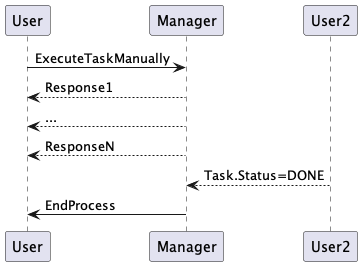
\includegraphics[height=0.3\textheight]{./part/Ejecucion/Seguimiento/MemoriaExplicativaDeCambios/img/1-ExecuteTaskManuallyInteraction}
    \caption{Use Case: 1-ExecuteTaskManuallyInteraction V2}\label{fig:1-ExecuteTaskManuallyInteractionV2}
\end{figure}

\begin{figure}[H]
    \centering
    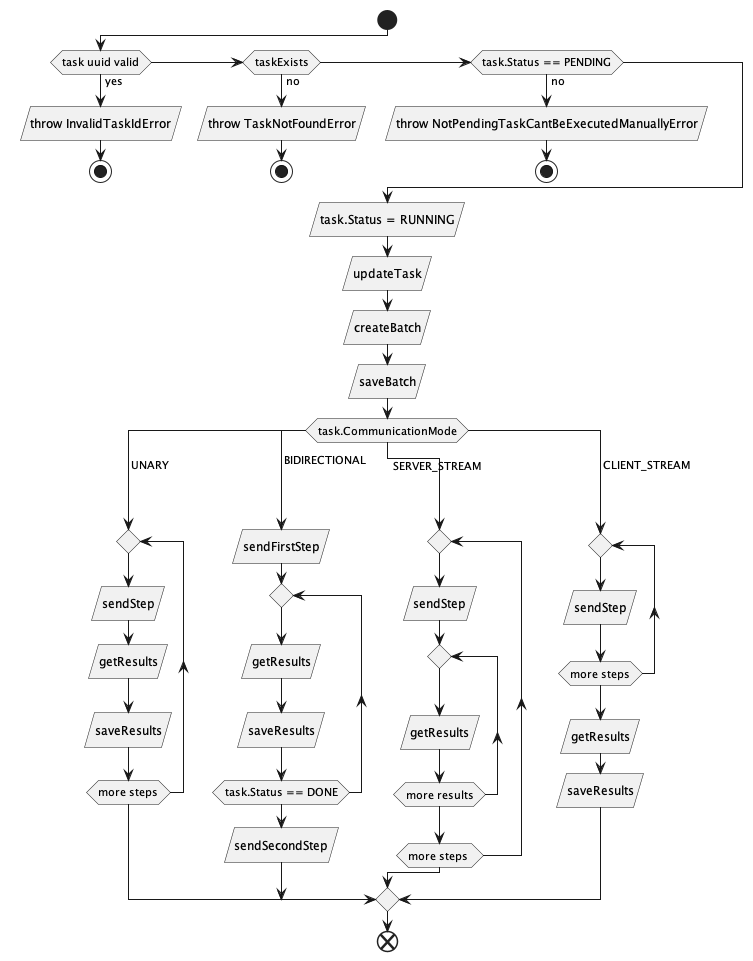
\includegraphics[height=0.55\textheight]{./part/Ejecucion/Seguimiento/MemoriaExplicativaDeCambios/img/1-TaskProcessor}
    \caption{Use Case: 1-TaskProcessor V2}\label{fig:1-TaskProcessorV2}
\end{figure}

\subsubsection{Caso práctico de las ventajas del \textit{DDD} y arquitectura de capas}

En el proceso de desarrollo se evaluó que el diseño original de separar el programa a ejecutar del cliente requería de una nueva implementación de intercomunicación que añadía complejidad y tiempo. Al ser un proyecto amplio y querer tocar todo el proceso de desarrollo no se ha visto interesante esa complejidad añadida. Por lo tanto se introdujo la lógica del programa de control dentro del programa cliente. Aquí se pudo ver la utilidad de la arquitectura al no encontrar ninguna fricción en este proceso. Dos programas con el mismo diseño estructural y organización para unirse o separarse sólo requiere mover archivos y no tocar código en sí.

El dominio se une sin tocarse el uno al otro ya que son idependientes todos los elementos. En la aplicación son casos de uso nuevos que tampoco interacciónan unos con otros. y la infraestructura lo mismo. Donde mejor se puede apreciar es en la estructura de carpetas de la figura

En el proyecto constará de 4 carpetas principales

\tiny
\dirtree{%
    .1 Project .
        .2 Domain.
        .2 Application.
        .2 Adapter.
        .2 Bootstrap.
}
\normalsize

\textbf{Dominio}

\begin{figure}[H]
    \tiny
\dirtree{%
    .1 Domain.
        .2 Step.
            .3 StepVo.
            .3 Repository.
                .4 consoleWrite.
            .3 Services.
                .4 Executor.
        .2 Result.
            .3 ResultVo.
}
\normalsize
    \caption[Diagrama de objetos de dominio]{}\label{fig:1-ClientDomainFolderStructure}
\end{figure}

\textbf{Aplicación}

\tiny
\dirtree{%
.1 Application.
    .2 Port.
        .3 in.
            .4 Step.
                .5 Execute.
                    .6 Command.
                    .6 UseCase.
}
\normalsize

\textbf{Adapters}

\tiny
\dirtree{%
    .1 Adapter.
        .2 in.
            .3 GRPC.
                .4 Harán uso de los useCases de aplicación cuando llegue una request RPC.
            .3 Console.
                .4 Por ejemplo si quisieramos ejecutar los casos de uso mediante terminal.
        .2 out.
            .3 console.
                .4 implementación de los repository de llamada a los servidores clientes.
}
\normalsize